\documentclass[tikz,border=8pt]{standalone}
% Shared look for every TikZ diagram. Load with \input{../../tools/tikz-style.tex}
\usepackage[T1]{fontenc}
\usepackage{lmodern}
\renewcommand{\sfdefault}{lmr}  % diagrams use the same serif as the text
\usetikzlibrary{arrows.meta, positioning, shapes.geometric, calc, fit, backgrounds}
\definecolor{cblue}{HTML}{4C78A8}
\definecolor{corange}{HTML}{F58518}
\definecolor{cgreen}{HTML}{54A24B}
\definecolor{cred}{HTML}{E45756}
\definecolor{cpurple}{HTML}{B279A2}
\definecolor{cgrey}{HTML}{6B6B6B}
\tikzset{
  every picture/.style={font=\sffamily, line width=1.2pt},
  box/.style={draw=#1, fill=#1!12, rounded corners=4pt, align=center, inner sep=7pt, minimum height=1.1cm},
  box/.default=cgrey,
  arrow/.style={-{Stealth[length=3mm]}, draw=cgrey, line width=1.4pt},
  title/.style={font=\sffamily\bfseries\Large},
  note/.style={font=\sffamily\small, text=cgrey, align=center},
}
\AtBeginDocument{\hyphenpenalty=10000 \exhyphenpenalty=10000}

% The running example: a hallway of 10 cells (1 m each), numbered 0-9, joined into a loop; doors at cells 1, 3 and 7.
% The robot stands in cell 1 but does not know it.
\definecolor{cbrown}{HTML}{9C755F}
\begin{document}
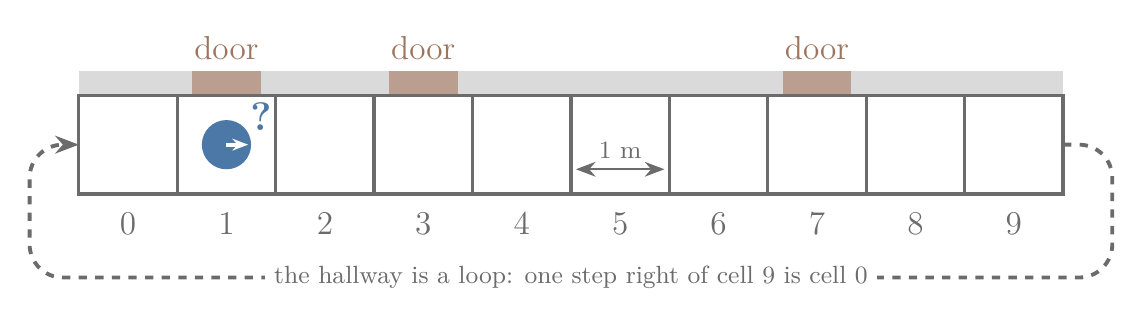
\begin{tikzpicture}[x=1.25cm, y=1.25cm, every node/.append style={font=\large}]
  % wall along the top, floor cells along the bottom
  \fill[cgrey!25] (0,1) rectangle (10,1.25);
  \foreach \d in {1,3,7} {
    \fill[cbrown!70] (\d+0.15,1) rectangle (\d+0.85,1.25);
    \node[cbrown, above] at (\d+0.5,1.25) {door};
  }
  \foreach \i in {0,...,9} {
    \draw[cgrey] (\i,0) rectangle (\i+1,1);
    \node[cgrey] at (\i+0.5,-0.3) {\i};
  }
  
  % loop: leaving cell 9 to the right enters cell 0
  \draw[arrow, cgrey, dashed, rounded corners=12pt] (10,0.5) -- (10.5,0.5) -- (10.5,-0.85) -- (-0.5,-0.85) -- (-0.5,0.5) -- (0,0.5);
  \node[note, fill=white] at (5,-0.85) {the hallway is a loop: one step right of cell 9 is cell 0};
  % robot
  \fill[cblue] (1.5,0.5) circle (0.25);
  \draw[-{Stealth[length=2mm]}, white, line width=1.5pt] (1.5,0.5) -- (1.72,0.5);
  \node[cblue, font=\bfseries\Large] at (1.85,0.78) {?};
  \draw[{Stealth[length=2.5mm]}-{Stealth[length=2.5mm]}, cgrey, line width=0.8pt] (5.05,0.25) -- (5.95,0.25) node[midway, above, note] {1 m};
\end{tikzpicture}
\end{document}
